\maketitle

\begin{abstract}
	In response to the critical need for efficient wildfire detection, this study presents an approach leveraging machine learning techniques applied to images from ground cameras and drones. Traditional methods, predominantly relying on satellite imagery, often need help with false positives and maintenance challenges. Our method addresses these limitations using a more direct and responsive visual data source. The significance of this research is underscored by California's substantial investment in wildfire management, with CalFire allocating \$3.3 billion annually for this purpose. The proposed system has the potential to significantly reduce costs and enhance early detection capabilities, particularly in remote areas.
    We curated a comprehensive dataset of 843,862 images, categorized into fire and non-fire classes, from a 16GB image repository from Kaggle. To optimize memory usage and enable efficient batch processing, we resized images to $200 \times 200$ pixels and removed duplicate images through image hashing. Data augmentation techniques expanded our dataset fivefold, including modifications in zoom, brightness, color jittering, Gaussian noise, and horizontal flipping. All images were standardized to JPEG format. For model development, we employed an 80\%-20\% split for training and testing and an 85\%-15\% split for training and validation. The study experimented with various neural networks, including ResNet, MobileNet, and AlexNet, over ten epochs using SGD and Adam optimization with a momentum of 0.9 and a learning rate of 0.001. ResNet emerged as the most effective model, benefiting from deeper layers and skip connections. MobileNet, while efficient, lacked the complexity needed for pattern recognition, and AlexNet's simpler architecture led to lower performance.
    To enhance the robustness of our model against overfitting, we are considering the implementation of k-fold cross-validation. Additionally, we plan to integrate semantic segmentation for more precise fire localization. Future work will focus on augmenting the dataset with edge case images, particularly those with various light sources, to improve the model's resistance to false positives. This research contributes to the wildfire detection field and demonstrates the potential of machine learning in addressing environmental and public safety challenges.
\end{abstract}

\section{Introduction}

In the realm of wildfire management and prevention, the development of an advanced early fire detection system stands as a critical innovation. Traditional methods, primarily relying on satellite imagery, are increasingly proving inadequate due to their susceptibility to false positives and ongoing maintenance challenges. To address these limitations, our research introduces a novel approach utilizing Computer Vision (CV) technology, harnessing images from ground-based cameras and drones. This methodology marks a significant leap in accurately identifying the presence of fire, particularly in its nascent stages.

The urgency and importance of this development are underscored by the efforts of organizations such as CalFire. As the state agency responsible for fire protection and the stewardship of over 31 million acres of California's wildlands, CalFire's expenditure of \$3.3 billion for wildfire protection and suppression vividly illustrates the substantial financial and environmental stakes involved. ~\citep{calfire} This immense budget not only highlights the state's commitment to managing and responding to wildfires but also reflects the enormous economic impact of these natural disasters.

In this context, the potential of an early fire detection system cannot be overstated. By enabling quicker and more accurate detection of wildfires, especially in remote or hard-to-reach areas where traditional surveillance methods are limited, such a system could have a profound economic effect. The anticipated benefits include significant cost savings, potentially amounting to millions of dollars annually, and more importantly, the mitigation of extensive environmental and property damage. Our research aims to explore and validate the effectiveness of this CV-based system, positioning it as a pivotal tool in the ongoing battle against wildfires.


Therefore, we decided to build a computer vision model that can classify a presense of fire from an image or a video. To develop a robust computer vision model for fire detection, we focused on utilizing ground-based imagery. This approach offers the dual benefits of real-time data acquisition and cost-effectiveness while ensuring high-resolution image quality. A key aspect of our methodology was the implementation of data augmentation techniques. These techniques enhance the model's ability to generalize by exposing it to a diverse array of fire scenarios, thereby improving its fire detection capabilities in various conditions.

Another critical component of our research was hyperparameter tuning. This process involved systematically adjusting the model's parameters to identify the most effective configuration. The optimal hyperparameter settings are crucial for maximizing the model's performance and accuracy in fire detection tasks.

To further enhance our model's capabilities, we integrated contextual information such as weather data and land use information. This integration enables the model to distinguish between different types of fires more effectively, leveraging the unique characteristics of each fire scenario.

A cornerstone of our approach was the use of pre-trained deep learning models, specifically ResNet, for feature extraction. These pre-trained models bring the advantage of established neural network architectures proven in various applications. Through transfer learning, we fine-tuned these models to better suit the specific needs of fire detection. This approach allowed us to capitalize on the advanced capabilities of pre-trained models while adapting them to the unique challenges of detecting fires in diverse environments.

\section{Literature Review}

\subsection{Deep Domain Adaptation Based Video Smoke Detection using Synthetic Smoke Images~\citep{Xu2017}}

This article used synthetic smoke images to train model to detect wildfire due to limited actual data.
We believed synthetic data would not capture true environmental situations so we used “fire” data and did not specify different subdomains of fire (such as wildfires).

\subsection{A Study on a Complex Flame and Smoke Detection Method Using Computer Vision Detection and Convolutional Neural Network
	~\citep{fire5040108}}

This article performed pre-processing using HSV color conversion, based on an image’s hue, saturation, and value to isolate a color region around the flame. Performing HSV color conversion proved to be computationally long and expensive, so we resorted to manipulation of other color attributes, such as color jittering.
	
\subsection{Wildfire Smoke Detection with Computer Vision
	~\citep{Daniel}}

This article explains in Section V, Part C: Increased the amount of material for training by applying mirror effect and exposure. We applied more data augmentation techniques to increase our dataset size even more, allowing it to generalize more types of situations.

\subsection{Image Data Augmentation Approaches: A Comprehensive Survey and Future directions~\citep{kumar2023image}}

This article discusses various data augmentation techniques applied to an image dataset and applied them in different computer vision tasks to compare their performances. It revealed the success of geometric data augmentation which translated and rotated an image, and non-geometric data augmentation, which flipped images and manipulated color. We applied these techniques to our model.

\subsection{A Robust Fire Detection Model via Convolution Neural Networks for Intelligent Robot Vision Sensing~\citep{s22082929}}

Traditional fire-detection methods would use smoke detection through smoke contours and the combination of ``color, texture and dynamic features.'' They further tracked a fire's motion by decomposing the fire images and applying an SVM to detect smoke.
These are vulnerable to false positives and objects that appear fire-like, so we applied deep learning via neural networks for fire detection since they are better at extracting features and creating high-level connections

\subsection{A Robust Fire Detection Model via Convolution Neural Networks for Intelligent Robot Vision Sensing~\citep{howard2017mobilenets}}

Due to resources available, we did not want a computationally expensive neural network to identify features from images. Upon research, we discovered that MobileNet implements a convolutional neural network that uses ``depthwise separable convolutions" to apply a single filter to each input channel, thus reducing ``the computation in the first few layers" and trading our model's accuracy for speed.

\subsection{Review of AlexNet for Medical Image Classification~\citep{tang2023review}}

This article explains: AlexNet first took advantage of deep convolutional neural networks for image detection after it won the 2012 ImageNet competition. Consisting of a large network structure with 60 million parameters and 650,000 neurons, it capitalizes on data augmentation and dropout methods to reduce overfitting. We decided to use this model as a baseline for our project.

\subsection{Deep Residual Learning for Image Recognition
	~\citep{he2015deep}}

This article explains: With very deep neural networks, performance may begin to degrade with increasing depth as gradients become smaller by backpropagation through more layers, thus preventing weights from being updated. ResNets solve this by introducing a residual learning framework which makes use of shortcut connections through which gradients can directly flow through each layer in the network. We adapt this architecture in our model.

\subsection{The effect of choosing optimizer algorithms to improve computer vision tasks: a comparative study~\citep{Hassan}}

This article reveals that the adam optimizer performs best for general computer vision tasks, especially for deep networks since it converges more quickly than stochastic gradient descent by adapting the learning rate during training. We decided to apply the adam optimizer in our ResNet model.

\subsection{A Comprehensive Survey of Loss Functions in Machine Learning~\citep{Wang2022}}

This article discusses and analyzes various loss functions and their performance in machine learning and deep learning tasks. As a binary classification problem, object detection performed well using a focal loss function, which adapts sigmoid cross entropy loss to resolve imbalance between classes. For our project, we decided to use sigmoid cross entropy loss based on its success in object detection on top of our dataset that was already roughly balanced between the fire and non-fire classes.

\section{Data Collection and Preprocessing}


\begin{figure}[htbp]
	\centering
	\subfloat[\centering Original]{{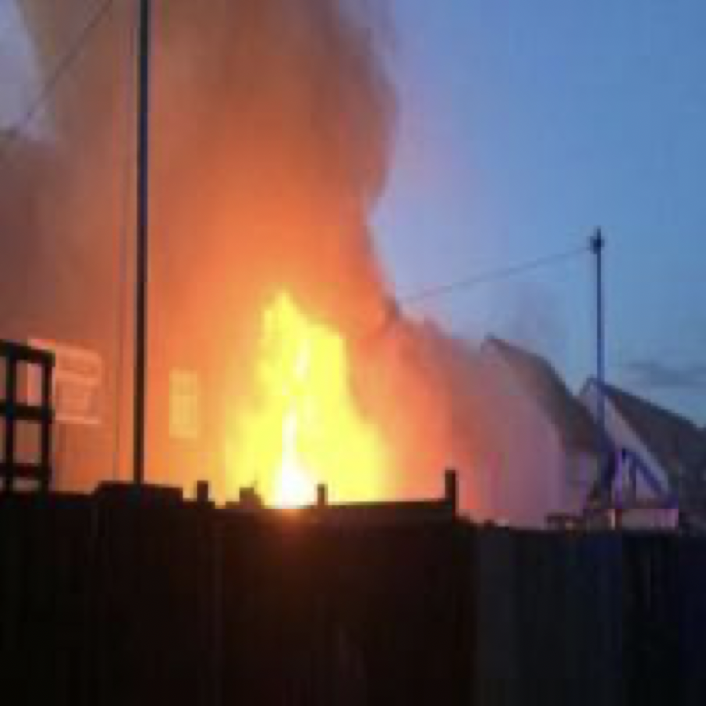
\includegraphics[width=2cm, height=2cm]{original} }}%
	\qquad
	\subfloat[\centering Brightened]{{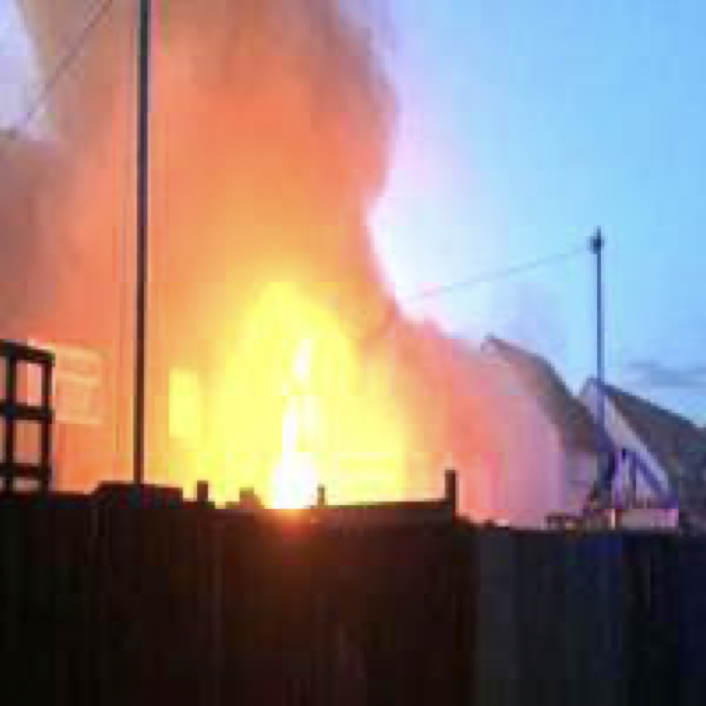
\includegraphics[width=2cm, height=2cm]{brightened} }}%
	\qquad
	\subfloat[\centering Noised]{{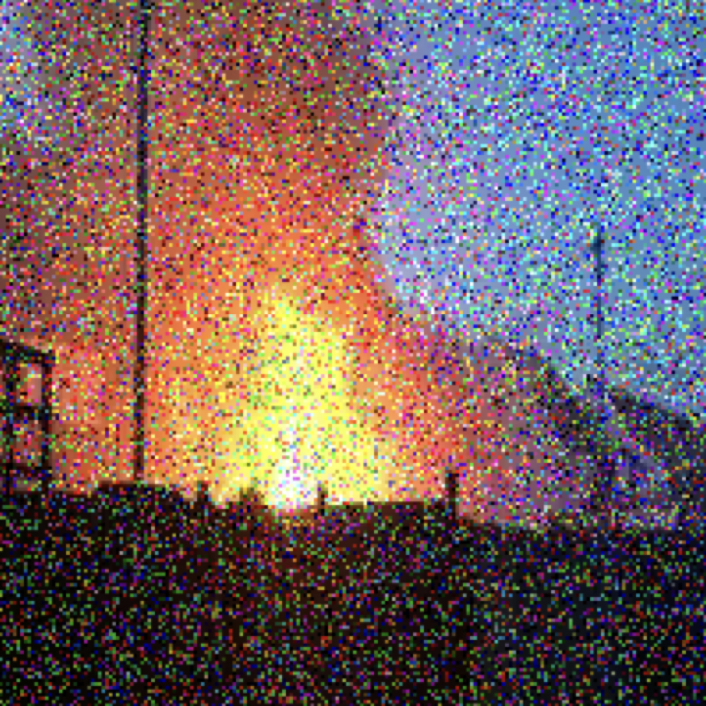
\includegraphics[width=2cm, height=2cm]{noised} }}%

	\subfloat[\centering Flipped]{{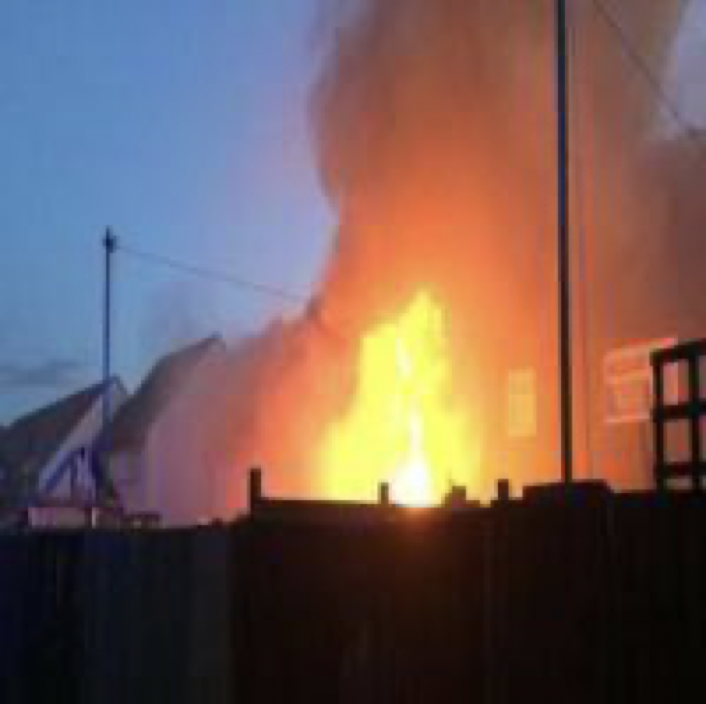
\includegraphics[width=2cm, height=2cm]{flipped} }}%
	\qquad
	\subfloat[\centering Jittered]{{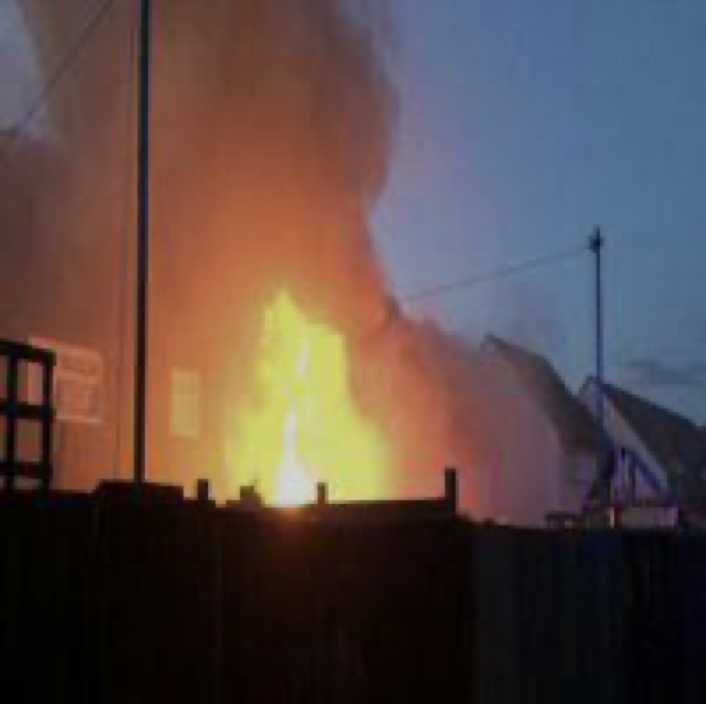
\includegraphics[width=2cm, height=2cm]{jittered} }}%
	\qquad
	\subfloat[\centering Zoomed]{{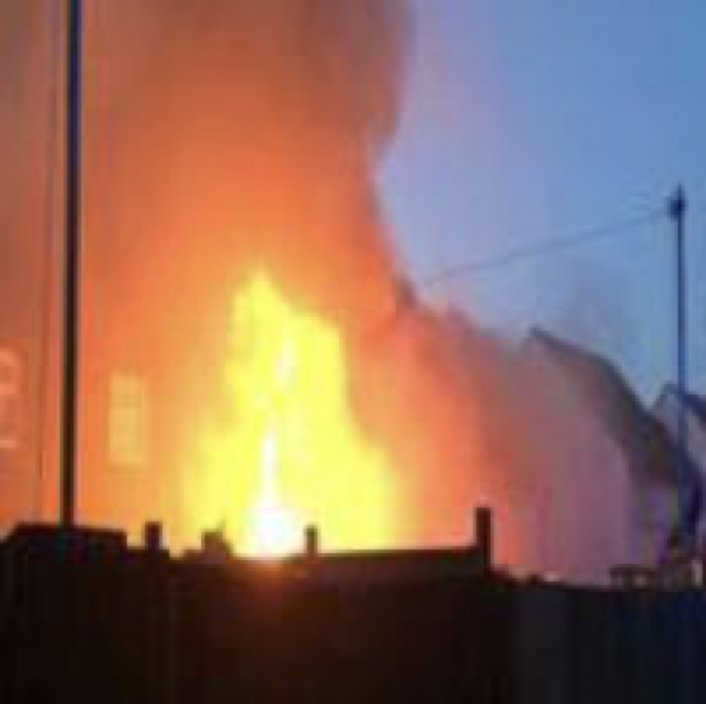
\includegraphics[width=2cm, height=2cm]{zoomed} }}%
	\caption{
		Example of augmented training data, using various methods
	}%
	\label{preprocessing}
\end{figure}

Our research leveraged a substantial 16GB image dataset, compiled from a range of Kaggle datasets and additional sources available on the internet. Among these were prominent collections such as \href{https://www.kaggle.com/datasets/mohnishsaiprasad/forest-fire-images}{Forest Fire Images}, \href{https://www.kaggle.com/datasets/ritupande/fire-detection-from-cctv}{Fire Detection from CCTV}, and \href{https://www.kaggle.com/datasets/diversisai/fire-segmentation-image-dataset}{Fire Segmentation Image Dataset}, along with several others, each contributing unique perspectives to our study.

We took several critical steps in preparing this dataset for analysis. Initially, all images were resized to a uniform dimension of \(200 \times 200\) pixels. This resizing was pivotal for enhancing memory efficiency, particularly beneficial for batch processing techniques in machine learning algorithms.

To maintain the quality and uniqueness of our dataset, we utilized advanced image hashing algorithms. This approach was instrumental in identifying and removing duplicate photos, including corrupted images, thus ensuring the purity and reliability of our dataset.

Further, we employed various data augmentation techniques to expand our dataset size by a factor of five. This augmentation included modifications in image attributes such as zoom levels, brightness adjustments, color jittering effects, the addition of Gaussian noise, and horizontal flipping. Such diversity in image transformations aimed to introduce a more robust set of features for model training, simulating a more comprehensive range of real-world scenarios. See figure \ref{preprocessing} for examples of these transformations.

A crucial aspect of our data processing was the standardization of the image file format. All images were converted to the JPEG format, a decision driven by JPEG's widespread compatibility and balance between quality and file size. We also implemented a systematic naming convention across all files to facilitate easier access and organization.

These extensive preprocessing efforts culminated in a well-structured dataset comprising two primary classes: fire images and non-fire images. The final counts stood at 462,980 images in the fire category and 380,882 in the non-fire category, offering a comprehensive resource for our subsequent analytical endeavors.

\section{Model and Methods}

We implemented a strategic approach to training and validating our models during our study. The dataset was divided into different subsets for training, testing, and validation purposes. Specifically, we adopted an 80\%-20\% split for the training and testing sets. This division ensured that a significant portion of the dataset was used for model training while retaining a substantial amount for testing purposes, thereby facilitating a comprehensive evaluation of model performance. Additionally, we employed an 85\%-15\% split between the training and validation sets for model validation.

We experimented with several architectures, notably ResNet, MobileNet, and AlexNet. Each of these networks has unique strengths and architectural characteristics, making them suitable for different image recognition tasks. ResNet, known for its deep architecture and residual learning framework, is particularly effective in avoiding the vanishing gradient problem. MobileNet, on the other hand, is designed for mobile and embedded vision applications, offering a good balance between efficiency and accuracy. AlexNet, one of the pioneer deep neural networks in image classification, has a simpler architecture and is known for its effectiveness in basic image recognition tasks. The comparative analysis of these networks was aimed at determining which model provided the best performance in terms of accuracy, computational efficiency, and generalizability in the context of our fire and non-fire image classification task.

The models were trained over ten epochs, which provided a balance between computational efficiency and allowing the models enough iterations to learn from the data effectively. We used the Stochastic Gradient Descent (SGD) optimizer for AlexNet and MobileNet, and the Adam optimizer for ResNet. The SGD was configured with a momentum of 0.9, which helps accelerate the optimizer in the relevant direction and dampens oscillations. We chose a learning rate (LR) of 0.001 to ensure gradual and stable convergence to the minimum loss.

\section{Results}

\begin{center}
	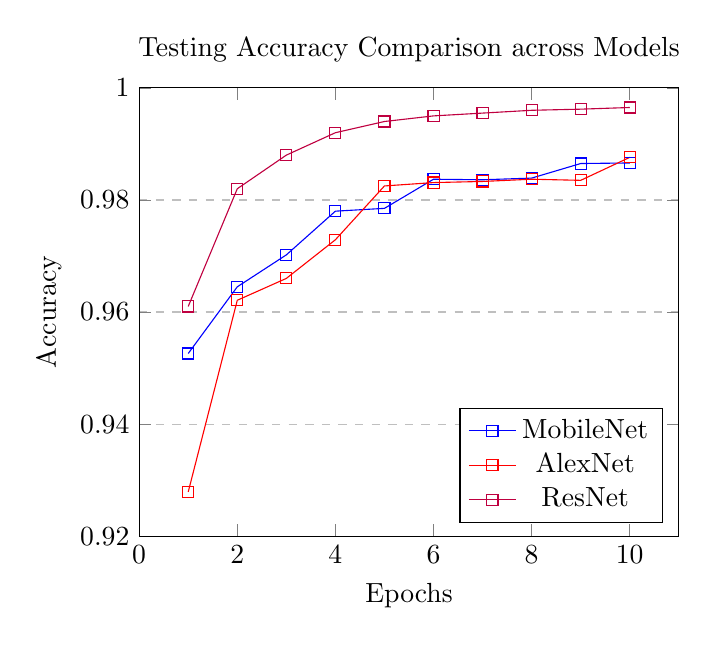
\begin{tikzpicture}
		\begin{axis}[
				title={Testing Accuracy Comparison across Models},
				xlabel={Epochs},
				ylabel={Accuracy},
				xmin=0, xmax=11,
				ymin=0.92, ymax=1,
				xtick={0,2,4,6,8,10},
				ytick={0.92, 0.94, 0.96, 0.98, 1},
				legend pos=south east,
				ymajorgrids=true,
				grid style=dashed,
			]

			\addplot[
				color=blue,
				mark=square,
			]
			coordinates {
					(1, 0.9526)
					(2, 0.9645)
					(3, 0.9702)
					(4, 0.978)
					(5, 0.9785)
					(6, 0.9837)
					(7, 0.9836)
					(8, 0.9839)
					(9, 0.9865)
					(10, 0.9866)
				};

			\addplot[
				color=red,
				mark=square,
			]
			coordinates {
					(1, 0.9279)
					(2, 0.9621)
					(3, 0.966)
					(4, 0.9729)
					(5, 0.9825)
					(6, 0.9831)
					(7, 0.9833)
					(8, 0.9837)
					(9, 0.9835)
					(10, 0.9876)
				};


			\addplot[
				color=purple,
				mark=square,
			]
			coordinates {
					(1, 0.961)
					(2, 0.982)
					(3, 0.988)
					(4, 0.992)
					(5, 0.994)
					(6, 0.995)
					(7, 0.9955)
					(8, 0.996)
					(9, 0.9962)
					(10, 0.9965)
				};
			\legend{MobileNet, AlexNet, ResNet}
		\end{axis}
	\end{tikzpicture}
\end{center}


Our experimental analysis yielded insightful results regarding the performance of different neural network architectures in fire and non-fire image classification. Among the models tested, ResNet emerged as the top-performing architecture. This superior performance can be attributed to its deeper layers and innovative use of skip connections. These skip connections facilitate the flow of gradients through the network, enabling the training of much deeper networks by effectively alleviating the vanishing gradient problem. Consequently, ResNet's ability to learn more complex patterns in the data was significantly enhanced, making it more adept at handling the intricacies of our diverse image dataset.

In contrast, MobileNet, while known for its efficiency in computational resource utilization, particularly in mobile and embedded device applications, did not perform as well as ResNet in our experiments. The streamlined architecture of MobileNet, designed for speed and low memory usage, seemingly compromised its ability to capture complex patterns within the images. This limitation was particularly evident when compared to ResNet's more intricate and deep architecture, which proved more capable of discerning nuanced features within our dataset.

Similarly, AlexNet's performance was also inferior to that of ResNet. Despite being one of the pioneering architectures in deep learning for image recognition, AlexNet's relatively more straightforward architecture seemed less equipped to handle our dataset's complexity than ResNet. AlexNet, with fewer convolutional layers and a more transparent structure, could have more effectively captured the detailed features required for accurate classification in our specific context.

These findings underscore the importance of the depth and complexity of neural network architectures in handling diverse and challenging datasets. ResNet's deep architecture with skip connections provided a significant edge in learning detailed and complex patterns, a crucial factor in our study's accurate classification of fire and non-fire images.


\section{Discussion}

In addressing the challenges posed by potential overfitting in our model, we are considering the implementation of k-fold cross-validation. This technique divides the dataset into \(k\) subsets, or `folds'. The model is then trained on \(k-1\) folds while using the remaining fold for testing. This process is repeated \(k\) times, with each fold as the testing set once. By training the model on different subsets of the data, k-fold cross-validation ensures a more robust and generalized learning, reducing the likelihood of overfitting.

Additionally, we plan to enhance our model's capability by integrating semantic segmentation. This advanced technique involves assigning labels to each pixel in an image, enabling the model to identify the precise regions where fire is present. Semantic segmentation is particularly effective in scenarios where understanding the context and exact location of the target within the image is crucial. By employing this method, our model will detect the presence of fire and delineate the specific areas affected by it.

Further, we aim to enrich our dataset with more edge case images to improve the model's accuracy and reduce false positives. These images will predominantly feature various light sources that could be mistaken for fire. By training the model on these additional images, we expect to enhance its ability to distinguish between actual fire and similar-looking light sources, making it more resilient to false-positive errors.

Collectively, we aim to refine the model's performance, ensuring it is accurate but also reliable and effective in diverse real-world scenarios.


\bibliography{iclr2023_conference}
\bibliographystyle{iclr2023_conference}

\subsubsection*{Acknowledgments}

We used the following Kaggle repositories to collect the images of fire.

\begin{itemize}
	\item \href{https://www.kaggle.com/datasets/mohnishsaiprasad/forest-fire-images}{Forest Fire Images}
	\item \href{https://www.kaggle.com/datasets/ritupande/fire-detection-from-cctv}{Fire Detection from CCTV}
	\item \href{https://www.kaggle.com/datasets/diversisai/fire-segmentation-image-dataset}{Fire Segmentation Image Dataset}
	\item \href{https://www.kaggle.com/datasets/elmadafri/the-wildfire-dataset}{The wildfire dataset}
	\item \href{https://www.kaggle.com/datasets/tharakan684/urecamain}{Fire Detection Using Surveillance Camera on Roads}
	\item \href{https://www.kaggle.com/datasets/alik05/forest-fire-dataset}{Forest Fire Dataset}
	\item \href{https://www.kaggle.com/datasets/brsdincer/wildfire-detection-image-data}{Wildfire Detection Image Data}
	\item \href{https://www.kaggle.com/datasets/ashutosh69/fire-and-smoke-dataset}{Fire and Smoke dataset}
	\item \href{https://www.kaggle.com/datasets/gondimjoaom/fire-images-database}{Fire Images Database}
	\item \href{https://www.kaggle.com/datasets/arbethi/forest-fire}{Forest Fire}
	\item \href{https://www.kaggle.com/datasets/parthmehta15/fire-gun}{Fire-Gun}
	\item \href{https://www.kaggle.com/datasets/christofel04/fire-detection-dataset}{Fire Detection Dataset}
	\item \href{https://www.kaggle.com/datasets/atulyakumar98/fire-and-gun-dataset}{Fire and Gun dataset}
	\item \href{https://www.kaggle.com/datasets/ashukr/wildfire}{Wild-fire}
	\item \href{https://www.kaggle.com/datasets/cristiancristancho/forest-fire-image-dataset}{Forest Fire Image Dataset}
	\item \href{https://www.kaggle.com/datasets/ahemateja19bec1025/wildfiresmokedatasetyolo}{WildFire-Smoke-Dataset-Yolo}
	\item \href{https://www.kaggle.com/datasets/kabilan03/fire-detection-dataset}{Fire detection dataset}
	\item \href{https://www.kaggle.com/datasets/ankan1998/fire-detection-in-yolo-format}{Fire Detection in YOLO format}
	\item \href{https://www.kaggle.com/datasets/ahemateja19bec1025/wildfiresmokedataset}{WildFire-Smoke-Dataset-Tensorflow}
\end{itemize}
